\documentclass{article}[12pt]
\renewcommand{\baselinestretch}{1.5}
\setlength{\parskip}{1em}

\usepackage[parfill]{parskip}
\usepackage[affil-it]{authblk}
\usepackage[space]{grffile}

\usepackage[a4paper]{geometry}
\usepackage[latin1]{inputenc}
\usepackage[english]{babel}

\geometry{verbose}
\usepackage{float}
\usepackage{graphicx}
\usepackage{setspace}
\usepackage{caption}

\usepackage{latexsym,textcomp,longtable,tabulary}
\usepackage{booktabs,array,multirow,braket}
\usepackage{amsfonts,amsmath,amssymb,mathbbol,calc,cancel}
\usepackage{subfigure,color,blindtext,enumitem,siunitx}
\usepackage[colorinlistoftodos]{todonotes}

\usepackage{mathtools}
\usepackage{url,hyperref,etoolbox}
\numberwithin{equation}{section}
\hypersetup{colorlinks=false,pdfborder={0 0 0}}

%+figure layout options
\restylefloat{figure}
\setlist{leftmargin=*,before=\setlength{\rightmargin}{\leftmargin}}
\graphicspath{{./figures/}{docs/figures/}}

\providecommand\citet{\cite}
\providecommand\citep{\cite}
\providecommand\citealt{\cite}

\makeatletter
\makeatother

\begin{document}
\newcommand{\rates}{F_{\theta}}
\newcommand{\tangent}{T_{\theta}}
\newcommand{\steadystates}{\partial S_{\theta}}

\newcommand{\Det}{\left| \frac{\partial\rates}{\partial u} \right|}
\newcommand{\measure}{\Psi_{\theta}}

\newcommand{\predictions}{\mathcal{P}}
\newcommand{\targets}{\mathcal{D}}
\newcommand{\loss}{L}

\newcommand{\Reals}{\mathbb{R}}

\title{Inference and Synthesis of\\ co-dimension one Bifurcations}
\author{Gregory Szep$^{1,2}$, Neil Dalchau$^2$ and Attila Csikasz-Nagy$^1$}
\affil{$^1$King's College London, $^2$Microsoft Research Cambridge}
\date{\today} \maketitle

\section{Introduction and Motivation}
\begin{itemize}
\item qualitative equivalence more important
\item fitting to time courses not appropriate
\item gradient information makes optimisation tractable
\item similar works
\end{itemize}
\clearpage

\section{Problem Statement}
Suppose we parameterise a set of differential equations for states $u\in\Reals^N$ with a function $\rates$ in an unknown parameter space $\theta\in\Reals^M$. We would like these differential equations to obey a set of target bifurcations $\targets:=\{p_1\dots p_K\}$ along a known bifurcation parameter $p\in\Reals$. The following sections outline how a gradient descent algorithm could encourage predicted bifurcations $\predictions(\theta)$ coming from parameterised differential equations to match specified targets $\targets$. This would allow us to design differential equations using high-level qualitative constraints and sample qualitatively equivalent models in regions of optimal $\theta$. Let the differential equations be defined as
\begin{align}
	\partial_t u=\rates(z)
	\qquad\mathrm{where}\quad z:=(u,p)\quad
	\rates : \Reals^{N+1}\rightarrow\Reals^N
	\label{eq:model}
\end{align}
\section{Methodology}
First we view the steady states of this problem in terms of implicit space curves \cite{Goldman2005CurvatureSurfaces} in an augmented state space $z\in\Reals^{N+1}$ which combines the state $u$ and bifurcation parameter $p$. We then realise that it is possible to analytically evaluate the curvature of the determinant $\Det(z)$, which when maximised encourages bifurcations in the region of $z$. In order to know which regions of $z$ need evaluation, a parameter continuation method \cite{Veltz2019PseudoArcLengthContinuation.jl,Farrell2016TheDiagrams} is used together with some pre-conditioning methods to ensure hyper-parameters remain constant. Finally a piecewise-differentiable semi-supervised objective function $\loss(\theta)$ is proposed that would allow gradient descent algorithms to efficiently encourage bifurcations and match their locations to targets $\targets$.

For clarity we guide the reader through the methods with the following co-dimension one normal forms: the saddle-node $\rates(z) = p + \theta_{1}u+\theta_{2}u^3$ and pitchfork $\rates(z) = \theta_{1} + p u+\theta_{2}u^3$ with corresponding targets $\targets$ as shown in Figure \ref{fig:saddle-node} and Figure \ref{fig:pitchfork} respectively. These figures show that the curvature of the determinant $\Det(z)$ increases in the vicinity of bifurcations and crosses zero at the bifurcation. This gives us our first hint of what should be optimised to encourage bifurcations. Success on these normal forms demonstrates the proof of concept, and success in practice is demonstrated on more complicated genetic feedback systems taken from examples in synthetic biology.
\begin{figure}[H]
\centering{}
\captionsetup{justification=centering}
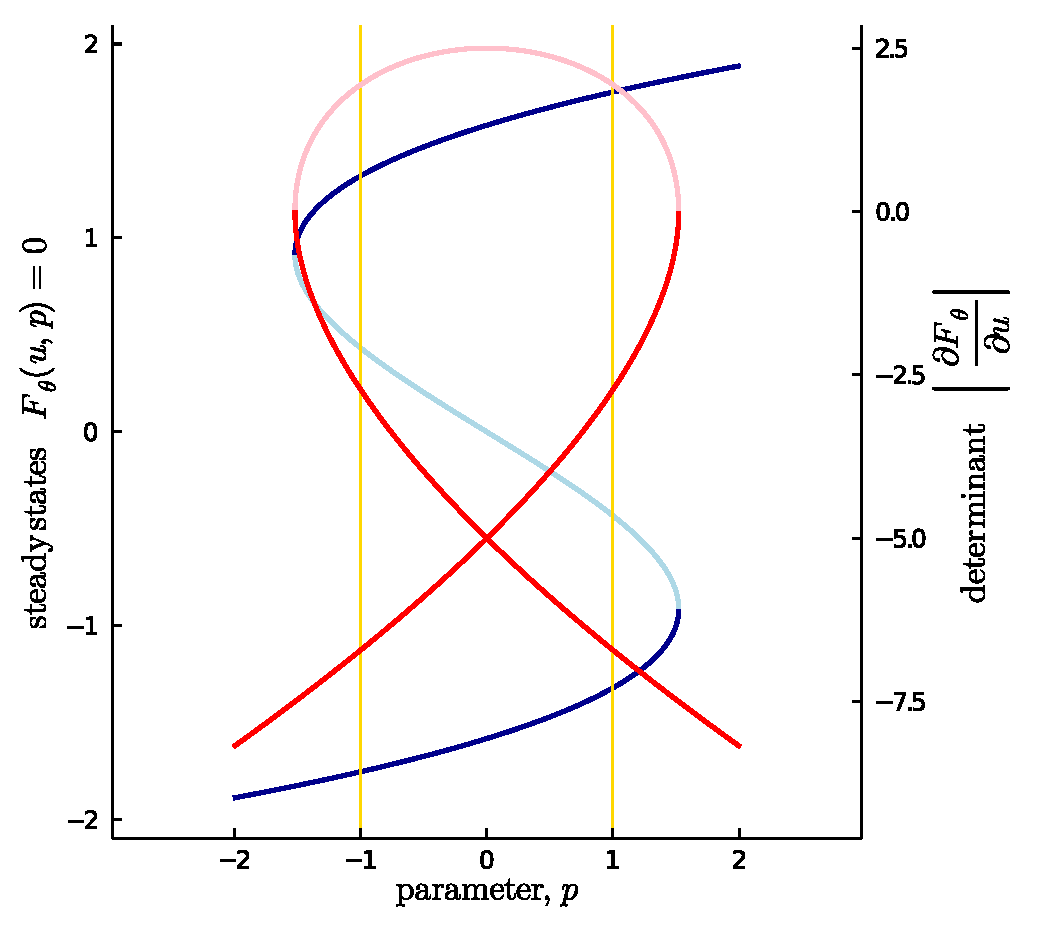
\includegraphics[width=11cm]{docs/figures/saddle-node}
\caption{Saddle-node normal form $\rates(z) = p + \theta_{1}u+\theta_{2}u^3$ with set $\theta=(2,-1)$ and targets $\targets=\{-1/2,1/2\}$. Lighter shades indicate the determinant crossing zero for unstable solutions}
\label{fig:saddle-node}
\end{figure}
\begin{figure}[H]
\centering{}
\captionsetup{justification=centering}
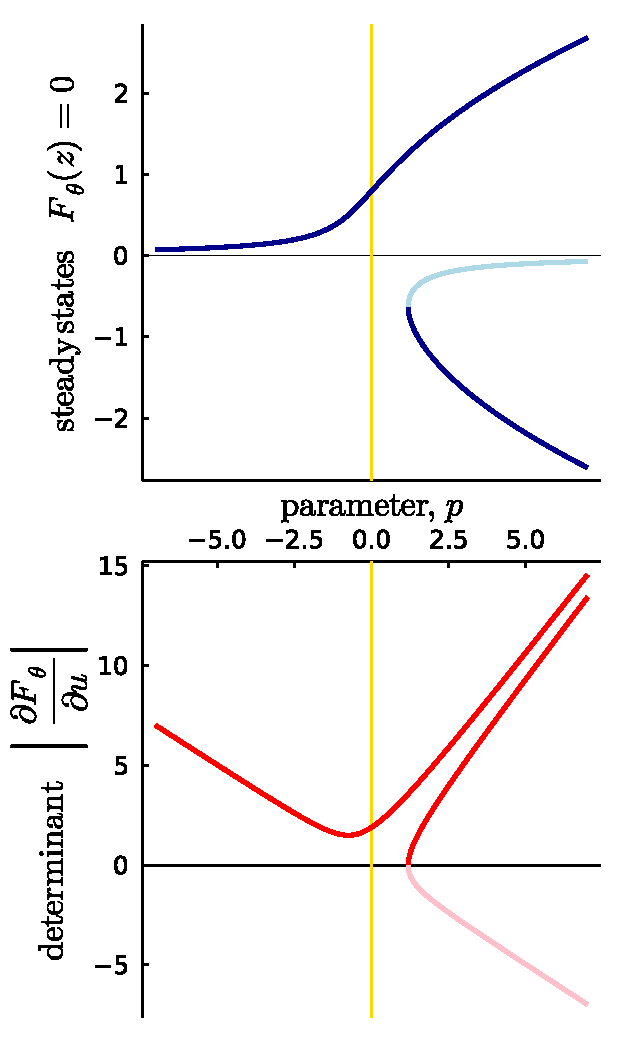
\includegraphics[width=11cm]{docs/figures/pitchfork}
\caption{Pitchfork normal form $\rates(z) = \theta_{1} + p u+\theta_{2}u^3$ with set $\theta=(-1/10,-1)$ and target $\targets=\{0\}$. Lighter shades indicate the determinant crossing zero for unstable solutions}
\label{fig:pitchfork}
\end{figure}

\subsection{Bifurcation Curves as Tangent Fields}
Obtaining a bifurcation curve involves solving for the steady states of \eqref{eq:model} along bifurcation parameter $p$. This is equivalent to finding the intersection between $N$ surfaces where each surface is given by a component of the rate function $\rates$. Each surface is embedded in $\Reals^{N+1}$ since the bifurcation parameter $p$ is an additional unknown variable. Thus the co-dimension one bifurcation curve is an $N+1$ dimensional implicit space curve defined by the $N$ equations
\begin{align}
    \rates(z) = 0
\end{align}

\begin{figure}[H]
\centering{}
\captionsetup{justification=centering}
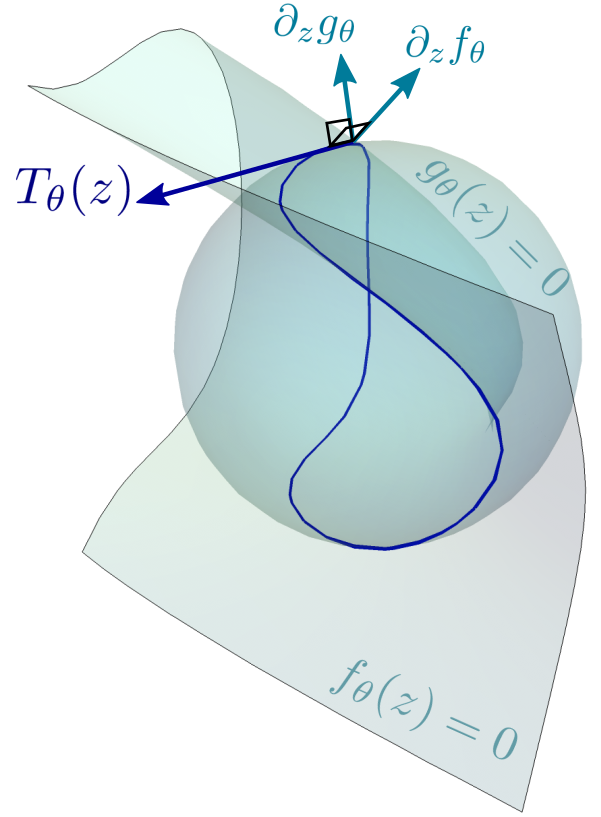
\includegraphics[width=6cm]{docs/figures/implicit-surfaces}
\caption{Two implicit surfaces $f_{\theta}(z)=0$ and $g_{\theta}(z)=0$ in $\mathbb{R}^3$ intersecting to form a\\ space curve which is tangent to field $\tangent(z)$ and perpendicular to gradients $\partial_{z}f_{\theta}$ and $\partial_{z}g_{\theta}$}
\label{fig:implicit-surfaces}
\end{figure}

An expression for the field $\tangent(z)$ tangent to the bifurcation curve would allow us to take derivatives and integrals along it. Fortunately the tangent field can be constructed by ensuring it is perpendicular to the gradient $\partial_z$ of each component of $\rates$ as illustrated by an example two component system in Figure \ref{fig:implicit-surfaces}. The tangent field $\tangent(z)$ can be constructed perpendicular to all gradient vectors using the properties of the determinant \cite{Goldman2005CurvatureSurfaces}
\begin{align}
    \tangent(z):=
    \left|\begin{matrix}
        \hat{z} \\
        \,\partial_{z}\rates\,
    \end{matrix}\right|
    \qquad\mathrm{where}\quad
    \hat{z}:=(\hat{u},\hat{p})\quad
	\tangent : \Reals^{N+1}\rightarrow\Reals^{N+1}
	\label{eq:tangent-field}
\end{align}
where $\hat{z}$ is a collection of unit basis vectors in the $\Reals^{N+1}$ space and $\partial_{z}\rates$ is an $N\times(N+1)$ augmented Jacobian matrix of partial derivatives including $\partial_p \rates$ in the last column. This construction ensures that the dot product of this field any gradient of a component of $\rates$
\begin{align}
    \tangent(z)\cdot\partial_z f_{\theta} =
    \left|\begin{matrix}
        \partial_z f_{\theta} \\
        \,\partial_{z}\rates\,
    \end{matrix}\right|
    \quad =0 \quad\forall f_{\theta}\in \rates
\end{align}
since the determinant of any matrix with two identical rows or columns is zero. Note that the tangent field $\tangent(z)$ is actually defined for all values of $z$ where adjacent field lines trace out other solutions where rates $\rates(z)\neq0$.

\begin{figure}[H]
\centering{}
\captionsetup{justification=centering}
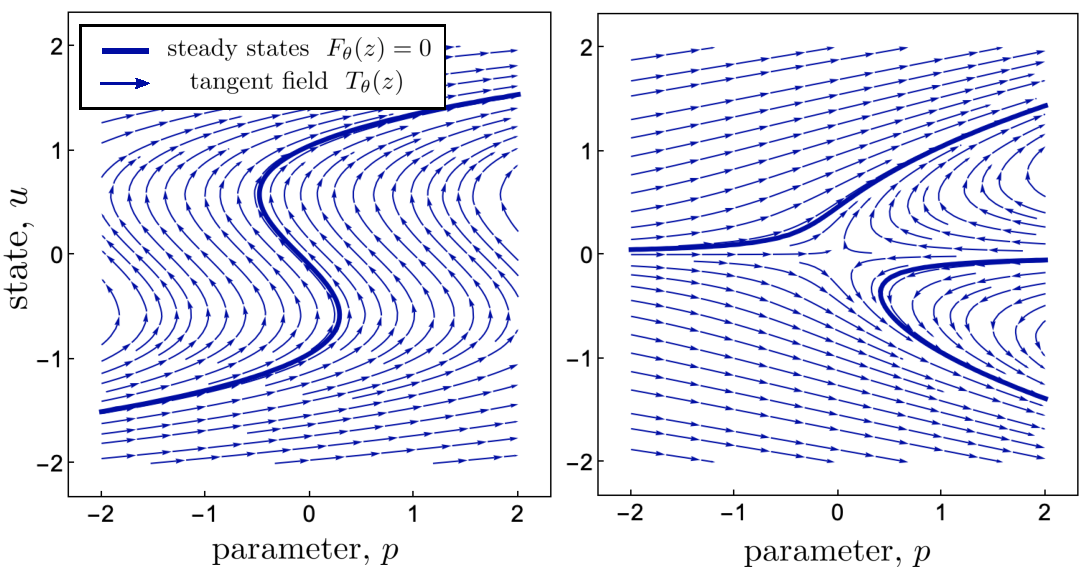
\includegraphics[width=14cm]{docs/figures/tangent-field}
\caption{Left/Right : Calculated tangent fields $\tangent(z)$ for the saddle-node/pitchfork normal forms for some set values of $\theta$ revealing that $\rates(z)=0$ picks out one of the traces in the field}
\label{fig:tangent-field}
\end{figure}

Figure \ref{fig:tangent-field} shows how the bifurcation curve defined by $\rates(z)=0$ picks out one of many traces in tangent field $\tangent(z)$ for the saddle and pitchfork. The tangent field $\tangent(z)$ can always be analytically evaluated by taking the determinant in \eqref{eq:tangent-field}. It becomes practical to proceed with calculations on $\tangent(z)$ in the whole space $z$ and pick out a single trace by solving $\rates(z)=0$ later. For the saddle-node and pitchfork respectively 
\begin{align}
    \tangent(z)=(\,3\theta_2 u^2-\theta_1\,)\,\hat{p}+\hat{u}
    \qquad\qquad
    \tangent(z)=(\,3\theta_2 u^2-p\,)\,\hat{p}+u\hat{u}
    \label{eq:tangent-field-examples}
\end{align}

\subsection{Evaluating Curvature of the Determinant}
Bifurcation points are defined as values of $z$ along the bifurcation curve where eigenvalues $\lambda$ of the Jacobian $\partial_u \rates(z)$ cross either the real or imaginary axis in the complex plane. Restricting our case to $\lambda\in\Reals$ for now, it would be sufficient to look for values of $z$ where one of the eigenvalues $\lambda$ crosses zero. Therefore the determinant of the Jacobian
\begin{align}
    \Det(z) := \big|\,\partial_u \rates\,\big|
\end{align}
crossing zero can be used as a readout of whether a bifurcation has occurred. Figure \ref{fig:determinant-curvature} reveals this is indeed also true for any value $z$ --- not just along $\rates(z)=0$ --- for the saddle-node and pitchfork. The tangent field $\tangent(z)$ only folds when $\Det(z)=0$. Plotting the value of the determinant along $\rates(z)=0$ from Figure \ref{fig:determinant-curvature} would give rise to Figures \ref{fig:saddle-node} and \ref{fig:pitchfork}.

\begin{figure}[H]
\centering{}
\captionsetup{justification=centering}
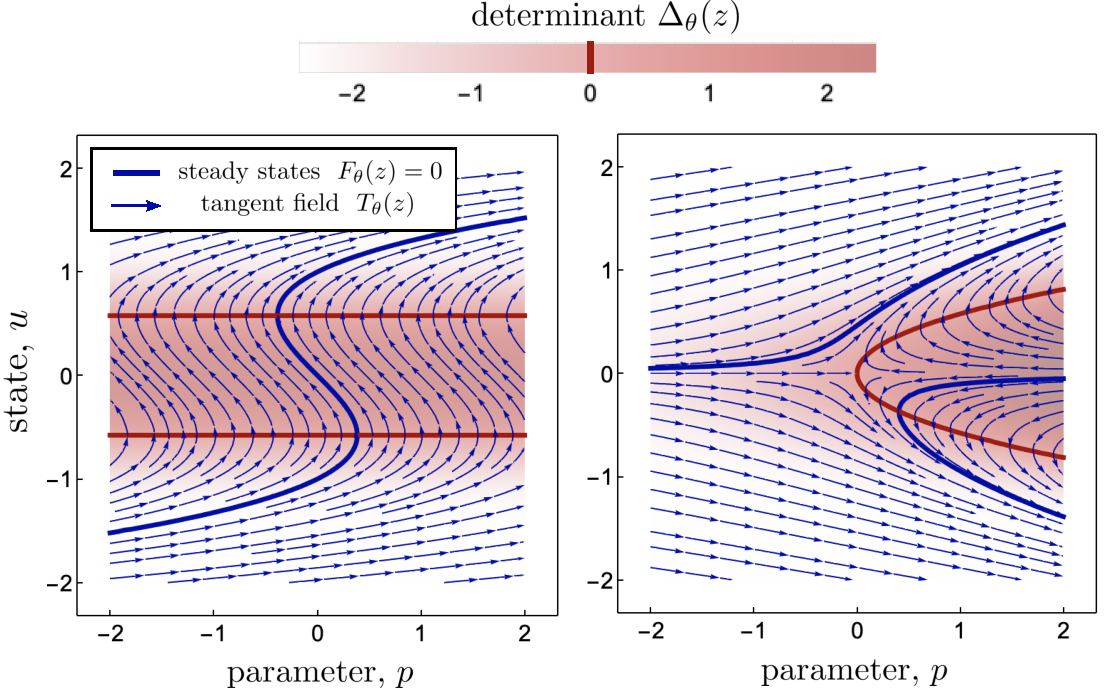
\includegraphics[width=14cm]{docs/figures/determinant-curvature}
\caption{Left/Right : Determinant $\Det(z)$ and tangent field $\tangent(z)$ for the saddle-node/pitchfork normal forms for some set values of $\theta$ revealing that $\Det(z)=0$ defines bifurcations}
\label{fig:determinant-curvature}
\end{figure}

Consequently the curvature of the determinant $\partial_{\tangent}^2\Det$ along the tangent field $\tangent(z)$ in the vicinity of bifurcations tends to increase. Fortunately this curvature can always be obtained in closed analytical form. The second directional derivative with respect to tangent field $\tangent(z)$
\begin{align}
    \partial_{\tangent}^2\Det &:=
    \bigg(
        \partial_z\left(
            \partial_z\Det \cdot \hat{\tangent}
        \right)
    \bigg)\cdot \hat{\tangent}\quad
    \mathrm{where} \quad \hat{\tangent}:=\frac{\tangent}{|\tangent|}\\
    &=
    \hat{\tangent}\cdot\partial_z^2\Det\cdot\hat{\tangent}
    \quad+\quad
    \partial_z\Det\cdot\partial_z\hat{\tangent}\cdot\hat{\tangent}
\end{align}
The first term in the expression above is the usual result involving the Hessian matrix $\partial_z^2\Det$ when taking second order directional derivatives. The second term involving the gradient $\partial_z\Det$ appears because $\hat{\tangent}(z)$ is a function of $z$ giving rise to a non-zero Jacobian matrix $\partial_z \hat{\tangent}$. Using expressions for tangent fields \eqref{eq:tangent-field-examples} and determinants for the saddle-node and pitchfork normal forms the determinant curvatures respectively become
\begin{align}
    \partial_{\tangent}^2\Det = 
    -\frac{6 \theta_2 \left(\theta _1^2-9 \theta _2^2 u^4+2\right)}
    {\left(\left(\theta _1+3 \theta _2 u^2\right){}^2+2\right){}^2}
    \qquad
    \partial_{\tangent}^2\Det =
    -\frac{2 u^2 \left(p+3 \theta _2 u^2\right) \left(9 \theta _2 \left(p+\theta _2 u^2\right)+2\right)}{\left(p^2+6 \theta _2 p u^2+9 \theta _2^2 u^4+2 u^2\right){}^2}
\end{align}
\subsection{Semi-supervised Objective Function}

This curvature of the determinant $\partial_{\tangent}^2\Det$ can be maximised to encourage bifurcations. For a particular bifurcation curve defined by $\rates(z)=0$ the total unsigned determinant curvature
\begin{align}
    \kappa(\theta) := \int_{\rates(z)=0}\!
    \big|\,\partial_{\tangent}^2\Det(z)\,\big|
    \,\mathrm{d}z
\end{align}
Here we note that the integrand as well as the limits are functions of $\theta$ and $z$. Once bifurcation points $\predictions(\theta)$ are present, the task is to match their locations to the targets $\targets$. However we do not know exactly now many bifurcations there for any given value of $\theta$ and there would be many different ways of satisfying the targets $\targets$. Therefore we borrow some concepts from electromagnetism and treat target locations as centres of attractive potentials and locations of predictions $\predictions(\theta)$ as interacting particles with a strong repulsive interaction.
\begin{align}
    L(\theta):= |\predictions(\theta)-\targets|
    -\log|\predictions(\theta)-\predictions(\theta)|
    -\log(1+\kappa(\theta))
\end{align}

\subsection{Hyper-parameter Preconditioning}


\section{Method}

\subsection{Pseudo-arclength Continuation}
\label{sec:continuation}

\begin{itemize}
    \item predictor-corrector algorithm
    \end{itemize}

\subsubsection{Optimization details}

\begin{itemize}
    \item ADAM
\end{itemize}

\section{Normal Forms}
\label{sec:normal-forms}

\begin{itemize}
    \item saddle-node, pitchfork, transcritical
    \item benchmarks against other algos
\end{itemize}


\section{Chemical Reaction Networks}
\label{sec:networks}

\begin{itemize}
    \item toggle switch
    \item cell cycle (Attila)
    \item application to structure $\rightarrow$ function (Luca)
\end{itemize}

\section{Conclusions and Extensions}
\label{sec:conclusions}

\begin{itemize}
    \item hyperparam optimization
    \item hopf bifurcations
    \item pattern formation in pdes (Neil)
\end{itemize}

\bibliography{refs}
\bibliographystyle{ieeetr}
\end{document}
